\documentclass[../main.tex]{subfiles}
\begin{document}
	
	\subsection{Характеристики оборудования}
	\begin{enumerate}
		\label{enu:comp}
		\item Компьютер:
		\begin{enumerate}
			\item Тип компьютера   Компьютер с ACPI на базе x64;
			\item Операционная система   Microsoft Windows 10 Pro.
		\end{enumerate}
		\item Системная плата:
		\begin{enumerate}
			\item тип ЦП   DualCore Intel Core i5-6200U, 2700 MHz (27 x 100);
			\item системная плата   HP 8079;
			\item чипсет системной платы   Intel Sunrise Point-LP, Intel Skylake-U;
			\item системная память   8072 МБ (DDR4 SDRAM).
		\end{enumerate}
	\end{enumerate}
	
	Замеры времени проводились для матриц размера 100х100, 200х200, 300х300, 400х400, 500х500. 
	Так как процессор, на котором выполнялись вычисления, имеет лишь 4 ядра, не было возможности произвести более обширное тестирование такое как, например, на GPU. 
	Тем не менее, распараллеливание вычислений оказалось эффективнее классического алгоритма, даже учитывая небольшое число ядер процессора.\\
	
	Очевидно, что производительность алгоритма на матрицах нечетного размера будет хуже, так как внутри алгоритма есть проверка на условие, после чего следует 2 вложенных цикла. 
	Они будут причиной увеличения времени работы. 
	Данное сравнение проводилось в лабораторной работе №2 и в данной работе производиться не будет.\\
	
	Замер времени проводился с помощью библиотеки time в Python 3.8 и метода processtime(). 
	На рисунке 1 видно, что во всех случаях попытка распараллелить алгоритм приводила к увеличению производительности алгоритма по времени и сокращению времени работы. \\
	
	Распараллеливание проводилось с помощью библиотеки threading для Python 3.8. Как показал опыт, данная библиотека оказалось недостаточно эффективной в сравнении с распараллеливанием на других языках. В среднем получилось уменьшить время работа на 10\% по сравнению с алгоритмом без распараллеливания. \\
	
	На момент замера времени работало в среднем 76 активных процессов.
	На графике отображено, что при нескольких процессах работа алгоритма будет дольше, чем при одном. 
	Это может зависеть от нескольких факторов таких, как: загруженность процессора другими процессами, обработка прерываний, ошибки внутри библиотеки для распараллеливания. \\
	
	\begin{figure}[H]
		\centering
		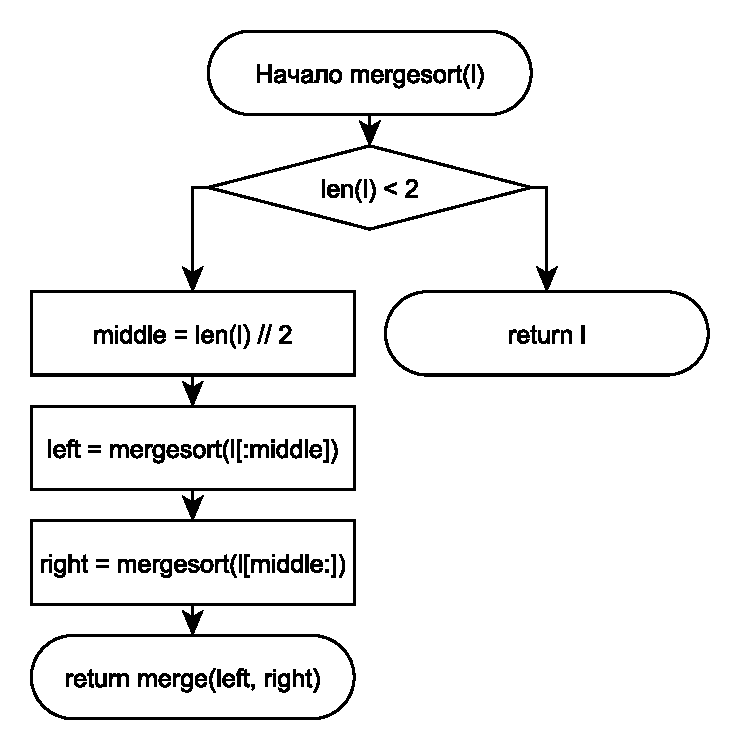
\includegraphics[width=0.7\linewidth]{img/1}
		\caption{Зависимость времени работы алгоритма Винограда от количества потоков}
		\label{fig:diss:1}
	\end{figure}

	\subsection{Вывод}
	
	В данном разделе указана характеристики оборудования на котором проводилось тестирование. 
	Указаны графики сравнения работы алгоритма в зависимости от количества потоков. 
	Подсчитано процентное соотношение скорости работы алгоритма в зависимости от количества потоков
	
\end{document}